\scanpage{108}
\mspage{107}%
motifs sur $\underline{C}$ prend ses valeurs en fait dans la catégorie des structures de Hodge (une polarisation d'une varéiét projective lisse $V$ définit canoniquement une polarisation de la structure de Hodge associée sur la cohomologie de Betti-Hodge). NB On n'a aucune idée sur ce que pourrait être l'image essentielle du foncteur précédent, par exemple s'il y a lieu d'espèrer qu'on trouve toutes les structures de Hodge (doncune équivalence de catégories : motifs sur $\underline{C}$ $\handwritten{\longrightarrow}$ structures de Hodge); cela semble peu probable, mais on n'a aucune indicationsérieuse dans un sens ou l'autre.

La catégorie des \deleted{pré} structures de Hodge est semi-simple. \deleted{En fait,} Si $G$ est le groupe de Galois d'une \inserted{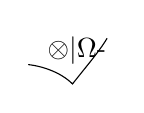
\begin{tikzpicture}[baseline=-.2ex,x=1em,y=1em]
\node[anchor=base west] at (0,.45) {$\unsure{\otimes|\Omega}$-};
\draw (-.35,.2) .. controls (.1,.15) and (.8,-.05) .. (1.25,-.5) .. controls (1.8,.2) and (2.2,.65) .. (2.5,1.15);
\end{tikzpicture}}catégorie \inserted{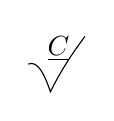
\begin{tikzpicture}[baseline=-.2ex,x=1em,y=1em]
\node[anchor=base west] at (0,.5) {$\underline{C}$};
\draw (-.35,.2) .. controls (0,.35) and (.25,-.2) .. (.45,-.8) .. controls (.75,-.2) and (1.1,.4) .. (1.7,1.2);
\end{tikzpicture}} de pré-structures de Hodge, à engendrement fini si on veut (pour simplifier), alors on peut expliciter en termes du groupe de Galois associé et de s\deleted{\unsure{e}}a\deleted{s} structure\deleted{s} $i_1\deleted{,\unsure{i_2}}$ ci-dessus la condition \deleted{que} pour que les objets de $\underline{C}$ soient en fait des structures de Hodge. Ceci est un exercice plaisant et délectable, qui devrait figurer dans un travail systématique sur les $\otimes$-catégories, dans le chapitre des exemples. On trouve des restrictions très sérieuses sur le groupe $G$ \deleted{(plus} muni de $i_1$ (en plus du fait que $G$ soit réductif).

4) Je laisse le soin à Saavedra de déterminer quelle structure supplémentaire on obtient sur la structure de Hodge ``complexe'' associée à une variété projective \inserted{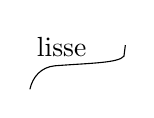
\begin{tikzpicture}[baseline=-.2ex,x=1em,y=1em]
\node[anchor=base west] at (0,.5) {lisse};
\draw (.1,-.7) .. controls (.2,-.25) and (.5,.1) .. (1,.15) .. controls (2.3,.25) and (3.3,.25) .. (3.5,.5) -- (3.55,.9);
\end{tikzpicture}} complexe $X$, lorsqu'on se donne cette dernière comme déduite d'une variété project\rlap{\raisebox{1.1ex}{\tikz[x=1em,y=1em]{\draw (0,0)--(0,.12) (0,.2)--(.01,.33) (.01,.43)--(.02,.49);}}}ive réelle $X_{\underline{R}}=X_o$.On trouve une notion de ``structure de Hodge réelle'', donnant naissance à une $\otimes$-catégorie correspondante. Dans le groupe de Galois motivique de celui-ci, en plus de la structure $i_1$, on trouve un élément $f_{\handwritten{\infty}}$ de $G(\underline{Q})$, \deleted{de degré} d'ordre 2 (jouant le rôle d'un ``élément de \rlap{f}Frobenius à l'infini''), qui correspond \margin{\tikz[x=1em,y=1em]{\draw (0,0) .. controls (.08,.02) and (.15,.13) .. (.2,.25);}}à l'automorphisme du foncteur de Betti $X_o\handwritten{\longmapsto} H^{\handwritten{*}}(X_o(\underline{C}),\underline{Q})$ déduit de l'homéomorphisme $x\handwritten{\mapsto}\overset{\handwritten{\rule{.55em}{.35pt}}}{x}$ de $X_o(\underline{C})$. Il faut expliciter les relations entre cet élément et $i_1$, $i_2$ !

